\documentclass[UTF8]{ctexart}
\usepackage{geometry}
\usepackage[backend=biber, style=authoryear]{biblatex} % 示例配置
\addbibresource{references.bib} % 替换为你的参考文献文件
\geometry{margin=1.5cm, vmargin={0pt,1cm}}
\setlength{\topmargin}{-1cm}
\setlength{\paperheight}{29.7cm}
\setlength{\textheight}{25.3cm}

% useful packages.
\usepackage{amsfonts}
\usepackage{amsmath}
\usepackage{amssymb}
\usepackage{amsthm}
\usepackage{enumerate}
\usepackage{graphicx}
\usepackage{multicol}
\usepackage{fancyhdr}
\usepackage{layout}
\usepackage{listings}
\usepackage{xcolor}
\lstset{language=C++}
\setlength{\headheight}{13pt}  % 增加头部高度
\usepackage{float, caption}

% Listings setting for code formatting
\lstset{
    basicstyle=\ttfamily,
    keywordstyle=\color{blue},
    commentstyle=\color{gray},
    stringstyle=\color{red},
    breaklines=true,
    frame=single,
    numbers=left,
    numberstyle=\tiny,
    stepnumber=1,
    tabsize=4
}

% some common commands
\newcommand{\dif}{\mathrm{d}}
\newcommand{\avg}[1]{\left\langle #1 \right\rangle}
\newcommand{\difFrac}[2]{\frac{\dif #1}{\dif #2}}
\newcommand{\pdfFrac}[2]{\frac{\partial #1}{\partial #2}}
\newcommand{\OFL}{\mathrm{OFL}}
\newcommand{\UFL}{\mathrm{UFL}}
\newcommand{\fl}{\mathrm{fl}}
\newcommand{\op}{\odot}
\newcommand{\Eabs}{E_{\mathrm{abs}}}
\newcommand{\Erel}{E_{\mathrm{rel}}}

\begin{document}

\pagestyle{fancy}
\fancyhead{}
\lhead{陈梓锐}
\chead{22435036}
\rhead{\today}


%\begin{abstract}
 %   The abstract is not necessary for the theoretical homework, 
   % but for the programming project, 
    %you are encouraged to write one.      
%\end{abstract}

% ============================================
\subsection*{如何使用}
在code中build文件下使用make命令编译，编译成功后，在build文件夹下会生成可执行文件P,在test目录下的test.josn调整初始条件即可使用不同的测试用例。

在网格数为64时求解非常慢，，请耐心等待。

\subsection*{设计文档}
本次大作业要求做五点差分格式在规则或不规则区域，dirichlet或neumann边界条件下求解的偏微分方程的数值解。
所以只需要求解五点差分格式的矩阵方程组，将得到的解转化成图片即可。

首先，当输入的网格大小为m时，在所有求解点矩阵
$
\begin{pmatrix}
u_{11} & u_{12} & \cdots & u_{1m} \\
u_{21} & u_{22} & \cdots & u_{2m} \\
\vdots & \vdots & \ddots & \vdots \\
u_{m1} & u_{m2} & \cdots & u_{mm}
\end{pmatrix}
$之外，包围了一圈边界点，即$
\begin{pmatrix}
    u_{00} & u_{01} & \cdots & u_{0m} &u_{0,m+1}\\
    u_{10} & u_{11} & \cdots & u_{1m} &u_{1,m+1}\\
    \vdots & \vdots & \ddots & \vdots & \vdots \\
    u_{m0} & u_{m1} & \cdots & u_{mm} &u_{m,m+1}\\
    u_{m+1,0} & u_{m+1,1} & \cdots & u_{m+1,m} &u_{m+1,m+1}
\end{pmatrix}$
边界点外面再包一圈ghost point，但并不显式的存储在矩阵中，用于计算Neumann边界条件。

在构造矩阵方程组时，只需要考虑内部的点，所以系数矩阵A是一个m阶方阵。

\subsection*{代码结构}
所有代码放在code文件夹中，头文件放在include文件夹中，源文件放在src文件夹中，build文件夹用于存放编译后的可执行文件，
opt中存放结果图片，test文件夹用于存放测试用例。


\subsection*{Problem $exp(y+sin(x))$}
考虑函数\begin{align}
    \left\{
        \begin{array}{ll}
            \Delta u(x,y) &= (\cos(x)\cos(x)-\sin(x)+1)\exp(y+\sin(x)) \quad (x,y)\in \Omega = (0,1) \times (0,1) \\
            u(x,y) &= \exp(y+\sin(x)) \quad (x,y)\in \partial \Omega = \{(0,y) \cup (1,y) \cup (x,0) \cup (x,1) \mid y \in [0,1], x \in [0,1]\}
        \end{array}
    \right.
\end{align}

在网格数为8,16,32,64的结果如下：

\begin{figure}[H]
    \centering
    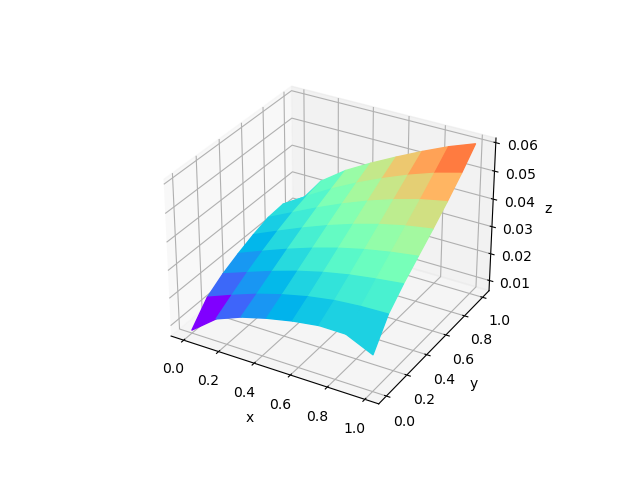
\includegraphics[width=0.2\textwidth]{pic/RD8.png}
    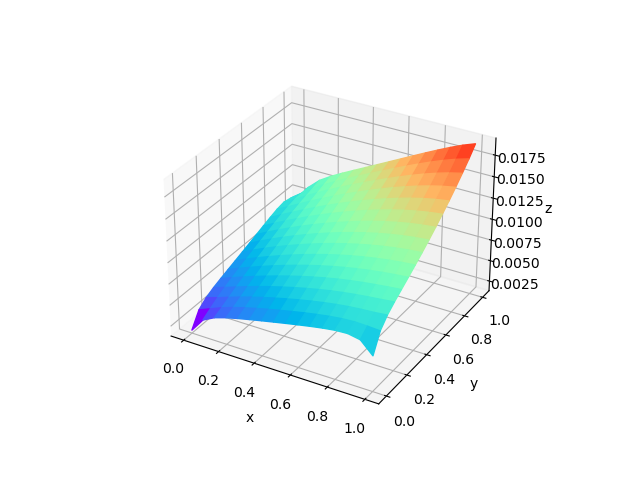
\includegraphics[width=0.2\textwidth]{pic/RD16.png}
    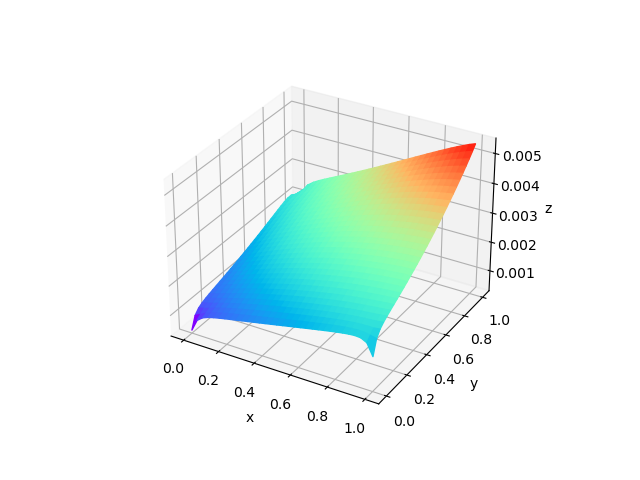
\includegraphics[width=0.2\textwidth]{pic/RD32.png}
    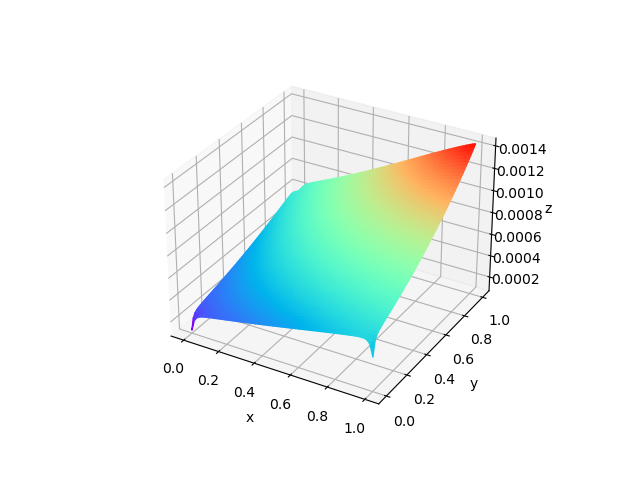
\includegraphics[width=0.2\textwidth]{pic/RD64.png}
    \caption{$exp(y+sin(x))$，规则网格数为8,16,32,64，Dirichlet边界。}
    \label{fig:RD}
\end{figure}
\begin{table}[H]
    \centering
    \begin{tabular}{c|cccc}
               &   $L_2$   &  $L_1$   &  $L_{\infty}$  \\
        
        8  &0.0920 &0.2315 &0.0605  \\
        
        16 &0.0404 &0.1484 &0.0190  \\
        
        32 &0.0159 &0.0840 &0.0054  \\

        64 &0.0059 &0.0446 &0.0014
    \end{tabular} 
\end{table}

\begin{figure}[H]
    \centering
    
\includegraphics[width=0.2\textwidth]{pic/ID8.png}
    
\includegraphics[width=0.2\textwidth]{pic/ID16.png}
    
\includegraphics[width=0.2\textwidth]{pic/ID32.png}
    
\includegraphics[width=0.2\textwidth]{pic/ID64.png}
    \caption{$exp(y+sin(x))$，不规则网格数为8,16,32,64，Dirichlet边界。}
    \label{fig:ID}
\end{figure}
\begin{table}[H]
    \centering
    \begin{tabular}{c|cccc}
               &   $L_2$   &  $L_1$   &  $L_{\infty}$  \\
        
        8  &0.0581 &0.1197 &0.0575  \\
        
        16 &0.0279 &0.0872 &0.0188  \\
        
        32 &0.0108 &0.0478 &0.0053  \\

        64 &0.0041 &0.0258 &0.0014
    \end{tabular} 
\end{table}

\begin{figure}[H]
    \centering
    
\includegraphics[width=0.2\textwidth]{pic/IN8.png}
    
\includegraphics[width=0.2\textwidth]{pic/IN16.png}
    
\includegraphics[width=0.2\textwidth]{pic/IN32.png}
    
\includegraphics[width=0.2\textwidth]{pic/IN64.png}
    \caption{$exp(y+sin(x))$，不规则网格数为8,16,32,64，Neumann边界。}
    \label{fig:IN}
\end{figure}
\begin{table}[H]
    \centering
    \begin{tabular}{c|cccc}
               &   $L_2$   &  $L_1$   &  $L_{\infty}$  \\
        
        8  &0.0069 &0.0157 &0.0049  \\
        
        16 &0.0036 &0.0125 &0.0017  \\
        
        32 &0.0012 &0.0058 &0.0004  \\

        64 &0.0004 &0.0031 &0.0001
    \end{tabular} 
\end{table}

%==========================================================================
%==========================================================================
\subsection*{自定义函数$sin(x*y)$}
考虑函数\begin{align}
    \left\{
        \begin{array}{ll}
            \Delta u(x,y) &= (x*x+y*y)*sin(x*y) \quad (x,y)\in \Omega = (0,1) \times (0,1) \\
            u(x,y) &= sin(x*y) \quad (x,y)\in \partial \Omega = \{(0,y) \cup (1,y) \cup (x,0) \cup (x,1) \mid y \in [0,1], x \in [0,1]\}
        \end{array}
    \right.
\end{align}
在网格数为8,16,32,64的结果如下：

\begin{figure}[H]
    \centering
    
\includegraphics[width=0.2\textwidth]{pic2/RD8.png}
    
\includegraphics[width=0.2\textwidth]{pic2/RD16.png}
    
\includegraphics[width=0.2\textwidth]{pic2/RD32.png}
    
\includegraphics[width=0.2\textwidth]{pic2/RD64.png}
    \caption{$exp(y+sin(x))$，规则网格数为8,16,32,64，Dirichlet边界。}
    \label{fig:RD}
\end{figure}
\begin{table}[H]
    \centering
    \begin{tabular}{c|cccc}
               &   $L_2$   &  $L_1$   &  $L_{\infty}$  \\
        
        8  &0.0081 &0.0169 &0.0078  \\
        
        16 &0.0037 &0.0112 &0.0025  \\
        
        32 &0.0015 &0.0064 &0.0007  \\

        64 &0.0005 &0.0034 &0.0001
    \end{tabular} 
\end{table}

\begin{figure}[H]
    \centering
    
\includegraphics[width=0.2\textwidth]{pic2/ID8.png}
    
\includegraphics[width=0.2\textwidth]{pic2/ID16.png}
    
\includegraphics[width=0.2\textwidth]{pic2/ID32.png}
    
\includegraphics[width=0.2\textwidth]{pic2/ID64.png}
    \caption{$exp(y+sin(x))$，不规则网格数为8,16,32,64，Dirichlet边界。}
    \label{fig:ID}
\end{figure}
\begin{table}[H]
    \centering
    \begin{tabular}{c|cccc}
               &   $L_2$   &  $L_1$   &  $L_{\infty}$  \\
        
        8  &0.0081 &0.0169 &0.0078  \\
        
        16 &0.0059 &0.0089 &0.0045  \\
        
        32 &0.0029 &0.0064 &0.0025  \\

        64 &0.0004 &0.0002 &0.0001
    \end{tabular} 
\end{table}

\begin{figure}[H]
    \centering
    
\includegraphics[width=0.2\textwidth]{pic2/IN8.png}
    
\includegraphics[width=0.2\textwidth]{pic2/IN16.png}
    
\includegraphics[width=0.2\textwidth]{pic2/IN32.png}
    
\includegraphics[width=0.2\textwidth]{pic2/IN64.png}
    \caption{$exp(y+sin(x))$，不规则网格数为8,16,32,64，Neumann边界。}
    \label{fig:IN}
\end{figure}
\begin{table}[H]
    \centering
    \begin{tabular}{c|cccc}
               &   $L_2$   &  $L_1$   &  $L_{\infty}$  \\
        
        8  &0.0041 &0.0068 &0.0054  \\
        
        16 &0.0022 &0.0057 &0.0020  \\
        
        32 &0.0008 &0.0028 &0.0056  \\

        64 &0.0003 &0.0015 &0.0001
    \end{tabular} 
\end{table}

%==========================================================
%==========================================================
\subsection*{自定义函数$exp(x*y)$}
考虑函数\begin{align}
    \left\{
        \begin{array}{ll}
            \Delta u(x,y) &= -(x*x+y*y)*exp(x*y) \quad (x,y)\in \Omega = (0,1) \times (0,1) \\
            u(x,y) &= exp(x*y) \quad (x,y)\in \partial \Omega = \{(0,y) \cup (1,y) \cup (x,0) \cup (x,1) \mid y \in [0,1], x \in [0,1]\}
        \end{array}
    \right.
\end{align}
在网格数为8,16,32,64的结果如下：

\begin{figure}[H]
    \centering
    
\includegraphics[width=0.2\textwidth]{pic3/RD8.png}
    
\includegraphics[width=0.2\textwidth]{pic3/RD16.png}
    
\includegraphics[width=0.2\textwidth]{pic3/RD32.png}
    
\includegraphics[width=0.2\textwidth]{pic3/RD64.png}
    \caption{$exp(y+sin(x))$，规则网格数为8,16,32,64，Dirichlet边界。}
    \label{fig:RD}
\end{figure}
\begin{table}[H]
    \centering
    \begin{tabular}{c|cccc}
               &   $L_2$   &  $L_1$   &  $L_{\infty}$  \\
        
        8  &0.0387 &0.1004 &0.0242  \\
        
        16 &0.0170 &0.0645 &0.0079  \\
        
        32 &0.0067 &0.0365 &0.0022  \\

        64 &0.0025 &0.0194 &0.0006
    \end{tabular} 
\end{table}

\begin{figure}[H]
    \centering
    
\includegraphics[width=0.2\textwidth]{pic3/ID8.png}
    
\includegraphics[width=0.2\textwidth]{pic3/ID16.png}
    
\includegraphics[width=0.2\textwidth]{pic3/ID32.png}
    
\includegraphics[width=0.2\textwidth]{pic3/ID64.png}
    \caption{$exp(y+sin(x))$，不规则网格数为8,16,32,64，Dirichlet边界。}
    \label{fig:ID}
\end{figure}
\begin{table}[H]
    \centering
    \begin{tabular}{c|cccc}
               &   $L_2$   &  $L_1$   &  $L_{\infty}$  \\
        
        8  &0.0245 &0.0538 &0.0231  \\
        
        16 &0.0119 &0.0391 &0.0078  \\
        
        32 &0.0046 &0.0215 &0.0022  \\

        64 &0.0017 &0.0116 &0.0006
    \end{tabular} 
\end{table}

\begin{figure}[H]
    \centering
    
\includegraphics[width=0.2\textwidth]{pic3/IN8.png}
    
\includegraphics[width=0.2\textwidth]{pic3/IN16.png}
    
\includegraphics[width=0.2\textwidth]{pic3/IN32.png}
    
\includegraphics[width=0.2\textwidth]{pic3/IN64.png}
    \caption{$exp(y+sin(x))$，不规则网格数为8,16,32,64，Neumann边界。}
    \label{fig:IN}
\end{figure}
\begin{table}[H]
    \centering
    \begin{tabular}{c|cccc}
               &   $L_2$   &  $L_1$   &  $L_{\infty}$  \\
        
        8  &0.0099 &0.0188 &0.0125  \\
        
        16 &0.0050 &0.0140 &0.0045  \\
        
        32 &0.0019 &0.0074 &0.0013  \\

        64 &0.0007 &0.0040 &0.0003
    \end{tabular} 
\end{table}

\subsection*{误差分析}
观察误差发现每次h增加一倍，误差减小一倍，说明格式是$O(h^2)$的。









% ===============================================

\end{document}